\documentclass[a4paper, 12pt]{article}

\newcommand{\languages}{english, french}

%%%%% Tools

\usepackage{comment}
\usepackage{lipsum}
\usepackage{xstring}

%%%%% Document

\usepackage{hyperref}
\usepackage{geometry}
\usepackage{fancyhdr}
\usepackage[parfill]{parskip}

\geometry{paper=a4paper,top=3.5cm,bottom=2.5cm,right=2.5cm,left=2.5cm}

\pagestyle{fancy}
\fancyhead[L]{}
\fancyhead[R]{\leftmark}
\fancyfoot[C]{\thepage}
\renewcommand{\headrulewidth}{0pt}

%%%%% Text

\usepackage[utf8]{inputenc}
\usepackage[T1]{fontenc}

\newlength{\mytextsize}
\makeatletter
\setlength{\mytextsize}{\f@size pt}
\makeatother

%%%%% Languages

\usepackage[\languages]{babel}

% english

\addto\captionsenglish{\def\figurename{Figure}}
\addto\captionsenglish{\def\tablename{Table}}

\newcommand{\st}{\text{s.t.}}

\IfStrEq{\languagename}{english}{
	\newcommand{\lgpreamble}{Preamble}
}

% french

\frenchbsetup{StandardLists=true}

\addto\captionsfrench{\def\figurename{Figure}}
\addto\captionsfrench{\def\tablename{Tableau}}
\addto\captionsfrench{\def\proofname{Preuve}}

\newcommand{\tq}{\text{t.q.}}
\newcommand{\cad}{c.-à-d. }
\newcommand{\Cad}{C.-à-d. }

\IfStrEq{\languagename}{french}{
	\newcommand{\lgpreamble}{Préambule}
}

%%%%% Styles

\usepackage[skip=\mytextsize]{caption}
\usepackage{float}
\usepackage{mdframed}
\usepackage{enumitem}
\usepackage{eurosym}
\usepackage{color}

\newcommand\caaption[1]{\caption{#1}\vspace{-1.5\mytextsize}}

%%%%% Mathematics

\usepackage{amsmath}
\usepackage{amssymb}
\usepackage{amsfonts}
\usepackage{bm}
\usepackage{esint}
\usepackage[makeroom]{cancel}

\newcommand{\fact}[1]{#1!}
\newcommand{\deriv}{\mathrm{d}}
\DeclareMathOperator{\tr}{tr}

%%%%% SI units

\usepackage[squaren,Gray,cdot]{SIunits}
\usepackage{sistyle}

\IfStrEq{\languagename}{french}{
	\SIdecimalsign{,}
}

%%%%% Chemistry

\usepackage[version=4]{mhchem}

%%%%% Table & Figure

\usepackage{array}
\usepackage{tabularx}
\usepackage{multirow}
\usepackage{multicol}
\newcolumntype{M}[1]{>{\centering\arraybackslash}m{#1}}
%\setlength\extrarowheight{0em}
\renewcommand{\arraystretch}{1.3}

\usepackage{pgfplots}
\usepackage{tikz}
\usetikzlibrary{shapes.geometric, positioning}
\usepackage{graphics}
\usepackage{graphicx}
\pgfplotsset{axis on top, compat = 1.3}

%%%%%% Theorems and Definitions

\usepackage{amsthm}
\usepackage{thmtools}

\IfStrEq{\languagename}{english}{
	\newcommand{\lgthm}{Theorem}
	\newcommand{\lglem}{Lemma}
	\newcommand{\lgprop}{Proposition}
	\newcommand{\lgdefn}{Definition}
	\newcommand{\lghyp}{Hypothesis}
	\newcommand{\lgquest}{Question}
	\newcommand{\lgansw}{Answer}
	\newcommand{\lgexpl}{Example}
	\newcommand{\lgrmk}{Remark}
	\newcommand{\lgnote}{Note}
	\newcommand{\lgtip}{Tip}
}

\IfStrEq{\languagename}{french}{
	\newcommand{\lgthm}{Théorème}
	\newcommand{\lglem}{Lemme}
	\newcommand{\lgprop}{Proposition}
	\newcommand{\lgdefn}{Définition}
	\newcommand{\lghyp}{Hypothèse}
	\newcommand{\lgquest}{Question}
	\newcommand{\lgansw}{Réponse}
	\newcommand{\lgexpl}{Exemple}
	\newcommand{\lgrmk}{Remarque}
	\newcommand{\lgnote}{Note}
	\newcommand{\lgtip}{Conseil}
}

\theoremstyle{plain}
\newtheorem{thm}{\lgthm}[section]
\newtheorem{lem}{\lglem}[section]
\newtheorem{prop}{\lgprop}[section]

\theoremstyle{definition}
\newtheorem{defn}{\lgdefn}[section]
\newtheorem{hyp}{\lghyp}[section]
\newtheorem{quest}{\lgquest}[]

\declaretheorem[
name=\lgansw,
qed={\lower-0.3ex\hbox{$\triangle$}},
within=quest
]{answ}

\declaretheorem[
name=\lgexpl,
qed={\lower-0.3ex\hbox{$\triangle$}},
within=section
]{expl}

\theoremstyle{remark}
\newtheorem*{rmk}{\lgrmk}
\newtheorem*{note}{\lgnote}
\newtheorem*{tip}{\lgtip}

\begingroup
\makeatletter
\@for\theoremstyle:=definition,remark,plain\do{%
	\expandafter\g@addto@macro\csname th@\theoremstyle\endcsname{%
		\addtolength\thm@preskip\parskip
	}%
}
\endgroup

%%%% Others

\renewcommand{\qedsymbol}{$\blacksquare$}

%%%%%%%%%%%%%%%%%%%

%%%%%%%%%%%%%%%%%%%

\title{Projet 2 - Ligne de production}
\newcommand{\subtitle}{Éléments du Calcul des Probabilités}
\author{François \textsc{Rozet} (s161024)\\Jules \textsc{Remes} (s162964)\\}
\newcommand{\context}{2\up{ème} année de Bachelier Ingénieur civil}
\date{Année académique 2017 - 2018}

%%%%%%%%%%%%%%%%%%%

\usepackage{colortbl}
\usepackage{listings}

\def\lstbasicfont{\fontfamily{pcr}\selectfont}

\lstdefinestyle{MatLab}{
	language=Matlab,
	%%%%%%
	showstringspaces=false,
	extendedchars=true,
	tabsize=4,
	columns=fixed,
	%%%%%%
	breaklines=true,
	breakatwhitespace=true,
	prebreak=\space,
	%%%%%%
	basicstyle=\fontfamily{pcr}\footnotesize,
	keywordstyle=\color{blue!60!black},
	commentstyle=\itshape\color{green!40!black},
	stringstyle=\color[rgb]{.627,.126,.941},
	%%%%%%
	morekeywords={ones, deal, ndims, shiftdim, circshift, permute, bsxfun, norminv, table, clearvars, getEsp, doSum},
	%%%%%%
	numbersep=0.5\mytextsize,
	numbers=left,
	numberstyle={\lstbasicfont\footnotesize},
	%%%%%%
	frame=single,
	rulecolor=\color{black},
	framexleftmargin=2\mytextsize,
	xleftmargin=2\mytextsize,
	captionpos=b,
	aboveskip=1\mytextsize,
	belowskip=1\mytextsize
}

\renewcommand{\thesubsection}{\thesection.\alph{subsection}}
\renewcommand{\thesubsubsection}{\thesubsection.\alph{subsubsection}}

\newcommand{\X}{\mathcal{X}}
\newcommand{\Y}{\mathcal{Y}}
\newcommand{\M}{\mathcal{M}}
\newcommand{\F}{\mathcal{F}}
\newcommand{\C}{\mathcal{C}}

%%%%%%%%%%%%%%%%%%%

\begin{document}
\newgeometry{margin = 2.5cm}
\makeatletter
\begin{titlepage}
	\begin{minipage}[t][0.425\textheight][t]{\textwidth}
		\begin{center}
			
\includegraphics[height=0.15\textheight]{include/resources/pdf/logo_uliege.pdf}
			\vfill
			{\huge \textsc{Université de Liège}}
			\vfill
		\end{center}
	\end{minipage}
	\vfill
	\begin{minipage}{\textwidth}
		\hspace{6pt}
		\begin{mdframed}[linewidth = 2pt, innertopmargin = 12pt, innerbottommargin = 12pt, leftline = false, rightline = false]
			\begin{center}
				{\huge \bfseries \@title}
			\end{center}
		\end{mdframed}
		\hspace{6pt}
	\end{minipage}
	\vfill
	\begin{minipage}[b][0.425\textheight][t]{\textwidth}
		\begin{center}
			\ifx\subtitle\undefined
			\else
			{\LARGE \subtitle}
			\fi
			\vfill
			{\large \@author}
			\vfill
			{\large \context \\[6pt] \@date}
		\end{center}
	\end{minipage}
\end{titlepage}
\makeatother
\restoregeometry
\newpage
\section{Manipulation des lois de probabilités}
\subsection{Lois de probabilités marginales}
Pour déterminer la probabilité qu'une variable aléatoire (discrète) $\X$ prenne une valeur spécifique de son domaine, il faut considérer tous les cas où elle prend cette valeur et additionner leur probabilité d'occurrence individuelle. \par
Ce processus est implémenté dans le script \texttt{Q1a.m}\footnote{Les scripts, et les fonctions qu'ils utilisent, sont disponibles dans l'annexe.} par le biais d'une contraction sommatoire sur deux indices. Les résultats sont exposés dans la(es) table(s) \ref{table:Q1a}.
\begin{table}[H]
	\centering
	\begin{tabular}{|c|c|}
		\hline
		$\M$ &     $P(\M)$      \\ \hline
		$1$  &  $\frac{7}{20}$  \\ \hline
		$2$  & $\frac{37}{100}$ \\ \hline
		$3$  &  $\frac{3}{25}$  \\ \hline
		$4$  &  $\frac{4}{25}$  \\ \hline
	\end{tabular}
	\hspace{2\mytextsize}
	\begin{tabular}{|c|c|}
		\hline
		$\F$ &     $P(\F)$      \\ \hline
		$1$  & $\frac{17}{50}$  \\ \hline
		$2$  & $\frac{31}{100}$ \\ \hline
		$3$  &  $\frac{7}{20}$  \\ \hline
	\end{tabular}
	\hspace{2\mytextsize}
	\begin{tabular}{|c|c|}
		\hline
		$\C$ &     $P(\C)$      \\ \hline
		$1$  &  $\frac{1}{5}$   \\ \hline
		$2$  & $\frac{31}{100}$ \\ \hline
		$3$  & $\frac{11}{50}$  \\ \hline
		$4$  &  $\frac{6}{25}$  \\ \hline
		$5$  & $\frac{3}{100}$  \\ \hline
	\end{tabular}
	\caaption{Lois de probabilités marginales des variables $\M$, $\F$ et $\C$.}
	\label{table:Q1a}
\end{table}
On remarque que les sommes des probabilités marginales associées aux valeurs respectivement admises par $\M$, $\F$ et $\C$ valent toutes $1$ vérifiant ainsi le second axiome de Kolmogorov.
\begin{align}
	\sum_{i} P(\X = x_i) & = 1
\end{align}
Puisque les trois axiomes sont établis, le premier et le troisième axiomes étant triviaux, il nous est permis d'utiliser les lois et théorèmes vus en cours pour étudier ce tableau dans le cadre du calcul de probabilité.
\subsection{Lois de probabilités conjointes}
De façon équivalente à la sous-question précédente, pour établir la probabilité qu'un couple de variables aléatoires (discrètes) $(\X,\Y)$ représente un point spécifique de leur plan, il suffit de sommer les probabilités d'occurrence de tous les cas où il le représente. \par
En exécutant le script \texttt{Q1b.m}, qui effectue une contraction sommatoire sur un seul indice, on obtient les valeurs contenues dans le(s) tableau(x) \ref{table:Q1b}.
\begin{table}[H]
	\begin{tabular}{|c|c|c|c|c|c|c|}
		\hline
		\multicolumn{2}{|c|}{\multirow{2}{*}{$P(\M,\C)$}} &                                        \multicolumn{5}{c|}{$\C$}                                        \\ \cline{3-7}
		\multicolumn{2}{|c|}{}                            &       $1$        &         $2$          &        $3$         &        $4$         &         $5$         \\ \hline
		\multirow{4}{*}{$\M$} &            $1$            & $\frac{7}{100}$  &  $\frac{217}{2000}$  & $\frac{77}{1000}$  &  $\frac{21}{250}$  &  $\frac{21}{2000}$  \\ \cline{2-7}
		                      &            $2$            & $\frac{37}{500}$ & $\frac{1147}{10000}$ & $\frac{407}{5000}$ & $\frac{111}{1250}$ & $\frac{111}{10000}$ \\ \cline{2-7}
		                      &            $3$            & $\frac{3}{125}$  &  $\frac{93}{2500}$   & $\frac{33}{1250}$  &  $\frac{18}{625}$  &  $\frac{9}{2500}$   \\ \cline{2-7}
		                      &            $4$            & $\frac{4}{125}$  &   $\frac{31}{625}$   &  $\frac{22}{625}$  &  $\frac{24}{625}$  &   $\frac{3}{625}$   \\ \hline
	\end{tabular}
	\hspace{0.5\mytextsize}
	\begin{tabular}{|c|c|c|c|c|}
		\hline
		\multicolumn{2}{|c|}{\multirow{2}{*}{$P(\M,\F)$}} &                   \multicolumn{3}{c|}{$\F$}                    \\ \cline{3-5}
		\multicolumn{2}{|c|}{}                            &        $1$         &         $2$          &        $3$         \\ \hline
		\multirow{4}{*}{$\M$} &            $1$            & $\frac{119}{1000}$ &  $\frac{217}{2000}$  &  $\frac{49}{400}$  \\ \cline{2-5}
		                      &            $2$            & $\frac{629}{5000}$ & $\frac{1147}{10000}$ & $\frac{259}{2000}$ \\ \cline{2-5}
		                      &            $3$            & $\frac{51}{1250}$  &  $\frac{93}{2500}$   &  $\frac{21}{500}$  \\ \cline{2-5}
		                      &            $4$            &  $\frac{34}{625}$  &   $\frac{31}{625}$   &  $\frac{7}{125}$   \\ \hline
	\end{tabular}
	\vspace{1\mytextsize} \newline
	\begin{tabular}{|c|c|c|c|c|c|c|}
		\hline
		\multicolumn{2}{|c|}{\multirow{2}{*}{$P(\F,\C)$}} &                                     \multicolumn{5}{c|}{$\C$}                                      \\ \cline{3-7}
		\multicolumn{2}{|c|}{}                            &       $1$        &        $2$         &        $3$         &        $4$         &       $5$        \\ \hline
		\multirow{3}{*}{$\F$} &            $1$            & $\frac{41}{500}$ & $\frac{527}{5000}$ & $\frac{407}{5000}$ & $\frac{81}{1250}$  & $\frac{4}{625}$  \\ \cline{2-7}
		                      &            $2$            & $\frac{8}{125}$  & $\frac{217}{2500}$ & $\frac{187}{2500}$ &  $\frac{51}{625}$  & $\frac{7}{2500}$ \\ \cline{2-7}
		                      &            $3$            & $\frac{27}{500}$ & $\frac{589}{5000}$ & $\frac{319}{5000}$ & $\frac{117}{1250}$ & $\frac{13}{625}$ \\ \hline
	\end{tabular}
	\caaption{Lois de probabilités conjointes une à une des variables $\M$, $\F$ et $\C$.}
	\label{table:Q1b}
\end{table}
On note que la somme de toutes les probabilités conjointes associées à une valeur fixe d'un des membres du couple est égale à la probabilité marginale de ce membre pour cette valeur.
\begin{align}
	\sum_{j} P(\X = x, \Y = y_j) & = P(\X = x)
\end{align}
\subsection{Lois de probabilités conditionnelles}{\label{sec:Q1c}}
Pour déterminer les lois de probabilités conditionnelles, nous avons développé l'expression originale de l'énoncé à partir de la relation suivante.
\begin{align}
	P(A|B) & = \frac{P(A) \cap P(B)}{P(B)}
\end{align}
Ainsi, on obtient une expression\footnote{Les expressions sont similaires pour $P(\F|\M,\C)$ et $P(\C|\M,\F)$.} facilement utilisable d'un point de vue numérique puisque autant le numérateur que le dénominateur sont connus.
\begin{align*}
	P(\M = x|\F = y,\C = z) & = \frac{P(\M = x) \cap P(\F = y,\C = z)}{P(\F = y,\C = z)} \\
	                        & = \frac{P(\M = x,\F = y,\C = z)}{P(\F = y,\C = z)}
\end{align*}
Pour simplifier le script \texttt{Q1c.m}, dont les résultats sont présentés dans la(es) table(s) \ref{table:Q1c}, nous avons utilisé la fonction \texttt{shiftdim} sur la matrice \texttt{MFC} pour nous permettre d'effectuer une division \og{}element-by-element\fg{} par le biais de la fonction \texttt{bsxfun}. Ce mécanisme est utilisé dans la plupart de nos scripts et il en est de même pour la contraction sommatoire sur les indices, déjà présente dans les premiers scripts.
\begin{table}[H]
	\centering
	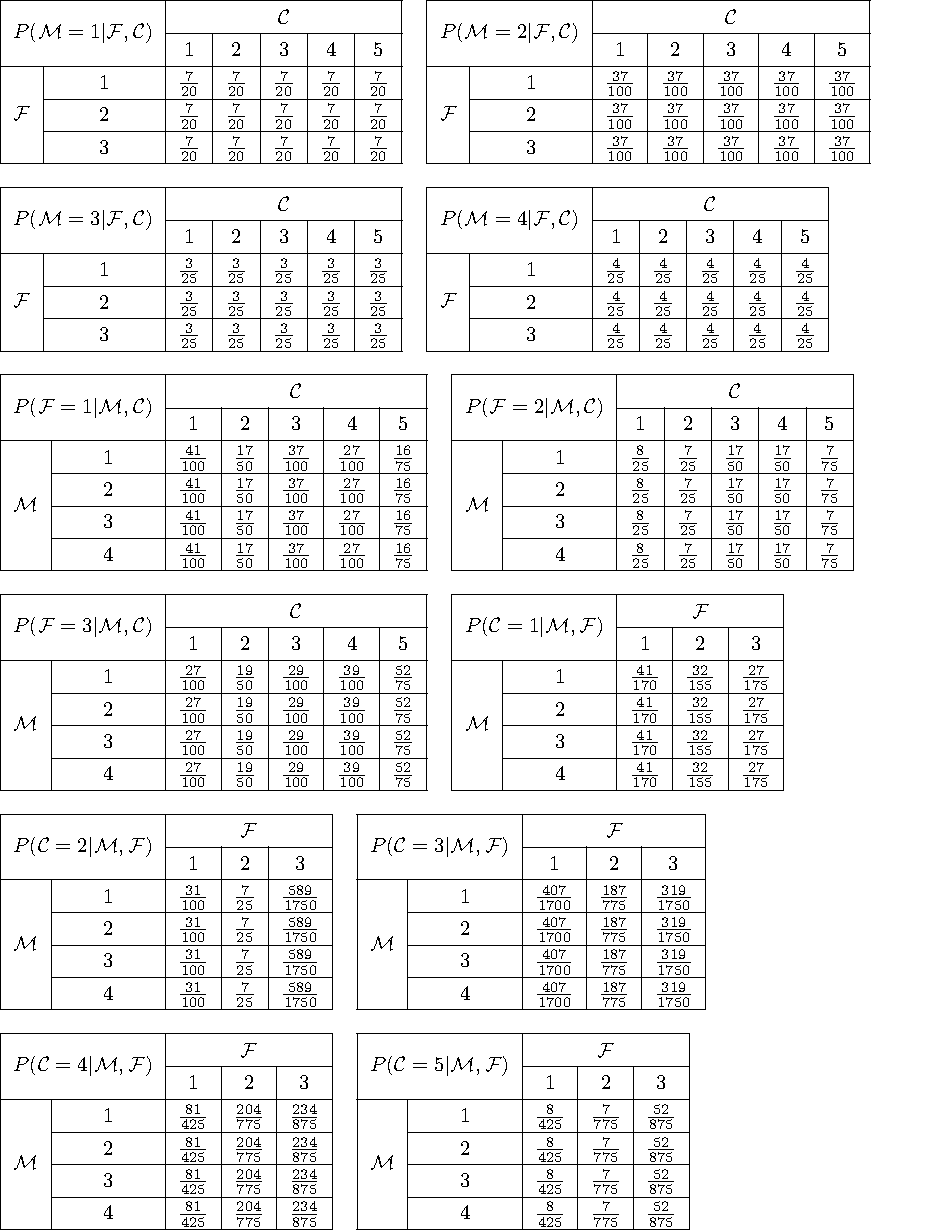
\includegraphics[width = 0.9\textwidth]{resources/table/Q1c/q1c.pdf}
	\caaption{Lois de probabilités conditionnelles des variables $\M$, $\F$ et $\C$.}
	\label{table:Q1c}
\end{table}
\subsection{Dépendance entre variables aléatoires}
En étudiant les résultats du script précédant, on peut affirmer que la variable	$\M$ est indépendante de $\F$ et de $\C$ mais que ces dernières sont inter-dépendantes.
\newpage
\section{Probabilités des pannes}
\subsection{Panne quelconque au cours du prochain moins}
L'usine sera en panne au cours du mois prochain si au moins une panne à lieu. Or, la probabilité qu'un évènement se produise est égal à $1$ diminué de la probabilité que l'évènement conjugué se produise.
\begin{align}
	P(A) & = 1 - P(\bar{A})
\end{align}
Dès lors la probabilité qu'au moins une panne ait lieu est égale à $1$ moins la probabilité qu'il n'y ait pas de panne\footnote{Voir l'implémentation dans le script \texttt{Q2a.m}.}.
\begin{align*}
	P(\textrm{panne}) & = 1 - P(\textrm{aucune panne}) \\
	                  & = 1 - \texttt{MFC}(1,1,1)   \\
	                  & = \num{0.9713}
\end{align*}
\subsection{Panne du processus de fermentation uniquement}
De la même manière que précédemment, la probabilité que le processus de fermentation soit soumis à une panne en sachant que les autres ne le seront pas est égale à $1$ diminué de la probabilité qu'il n'y soit pas soumis sous les mêmes conditions\footnote{Voir l'implémentation dans le script \texttt{Q2b.m}.}. Or, cette dernière valeur, nous l'avons déjà calculée dans la section \ref{sec:Q1c} (cf. table \ref{table:Q1c}).
\begin{align*}
	P(\F \neq 1|\M = 1, \C = 1) & = 1 - P(\F = 1|\M = 1, \C = 1) \\
	                            & = \num{0.59}
\end{align*}
\newpage
\section{Coût moyen des pannes}
\subsection{Coûts moyens de réparation}
Le coût moyen lié à la nécessité de réparer une machine est, en fait, la définition de l'espérance liée à ce coût. Dès lors, pour l'obtenir, il suffit de calculer cette dernière.
\begin{align}
	E\left\{\X\right\} & = \sum_{i} x_i P(\X = x_i)
\end{align}
Pour ce faire, nous avons implémenté une fonction \texttt{getEsp} qui calcule cette somme à partir d'une matrice\footnote{Une matrice de dimension $n$.} des gains et de la matrice de leur probabilité respective. \par
Il nous est aussi demandé explicitement de calculer la variance du coût ce que nous faisons à partir d'une relation dérivée de sa définition.
\begin{align}
	V\left\{\X\right\} & = E\left\{\left(X - E\left\{X\right\}\right)^2\right\}                                                                               \\
	                   & = \sum_{i} \left(x_i - E\left\{X\right\}\right)^2 P(\X = x_i) \nonumber                                                              \\
	                   & = \sum_{i} {x_i}^2 P(\X = x_i) - 2 E\left\{X\right\} \sum_{i} {x_i} P(\X = x_i) + E\left\{X\right\}^2 \sum_{i} P(\X = x_i) \nonumber \\
	                   & = E\left\{X^2\right\} - \bcancel{2} E\left\{X\right\}E\left\{X\right\} + \bcancel{E\left\{X\right\}^2} \nonumber                     \\
	                   & = E\left\{X^2\right\} - E\left\{X\right\}^2
\end{align}
Les coûts nous étant fournis et leur probabilité marginale étant connue (cf. table \ref{table:Q1a}), on les utilise directement dans le script \texttt{Q3a.m} pour obtenir les résultats suivants.
\begin{table}[H]
	\centering
	\begin{tabular}{|c|c|c|c|}
		\hline
		                         $\X$                          & $\mathcal{K}_\M$  & $\mathcal{K}_\F$  &  $\mathcal{K}_\C$  \\ \hline
		 $E\left\{\X\right\}$ $\left[\textrm{\euro{}}\right]$  &  $\num{7.76e3}$   &  $\num{9.09e3}$   &  $\num{2.879e4}$   \\ \hline
		$V\left\{\X\right\}$ $\left[\textrm{\euro{}}^2\right]$ & $\num{4.23024e7}$ & $\num{5.58819e7}$ & $\num{3.955059e8}$ \\ \hline
	\end{tabular}
	\caaption{Espérance et variance des coûts de réparation pour chaque machine.}
	\label{table:Q3a}
\end{table}
\subsection{Espérance de la fonction coût}
\begin{enumerate}[label=\roman*.]
	\item Puisque nous connaissons les vecteurs coûts de chaque machine, il est facile de construire la matrice $\Phi$ dans laquelle chaque configuration possible est représentée. Par simplicité, dans le script \texttt{Q3b.m}, nous donnons à cette matrice la même forme que la matrice \texttt{MFC} qui est, par ailleurs, la matrice des probabilités respectives aux éléments de $\Phi$. \par
	Ensuite, comme à la question précédente, on applique \texttt{getEsp} sur $\Phi$ et $\texttt{MFC}$ ce qui nous donne les valeurs du tableau \ref{table:Q3b}.
	\begin{table}[H]
		\centering
		\begin{tabular}{|c|c|}
			\hline
			                         $\X$                          &       $\phi$       \\ \hline
			 $E\left\{\X\right\}$ $\left[\textrm{\euro{}}\right]$  &  $\num{4.564e4}$   \\ \hline
			$V\left\{\X\right\}$ $\left[\textrm{\euro{}}^2\right]$ & $\num{5.325216e8}$ \\ \hline
		\end{tabular}
		\caaption{Espérance et variance de la fonction coût.}
		\label{table:Q3b}
	\end{table}
	\item Concrètement, cette espérance représente le coût en réparation que l'entreprise \textit{Bièrenoulli} devra payer chaque mois en moyenne.
	\item On sait que l'espérance d'une somme de variables aléatoires est égale à la somme des espérances de chaque variable.
	\begin{align}
		E\left\{\sum_{i} \X_i\right\} & = \sum_{i} E\left\{\X_i\right\}
	\end{align}
	Dès lors, puisque la fonction coût est déterminée par la somme de trois coûts, son espérance est égale à la somme des espérances individuelles de chaque coût.
	\begin{align*}
		E\left\{\phi\right\} & = E\left\{\mathcal{K}_\M + \mathcal{K}_\F + \mathcal{K}_\C\right\}                                 \\
		                     & = E\left\{\mathcal{K}_\M\right\} + E\left\{\mathcal{K}_\F\right\} + E\left\{\mathcal{K}_\C\right\}
	\end{align*}
	Cette relation est vérifiée par les calculs. \par
	Quant à elle, la variance d'une somme de variables aléatoires est égale à la double somme de leurs covariances\footnote{D'après la définition de la covariance, lorsque $\X$ et $\Y$ sont égaux, elle est égale à leur variance.} une à une.
	\begin{comment}
	\begin{alignat}{2}
		                  &  & \operatorname{cov}(\X,\Y) & = \sum_{i} \sum_{j} x_i y_j P(\X = x_i,\Y = y_j) - E\left\{\X\right\} E\left\{\Y\right\} \\
		\Rightarrow \quad &  & \operatorname{cov}(\X,\X) & = \sum_{i} \sum_{j} x_i x_j P(\X = x_i,\X = x_j) - E\left\{\X\right\}^2 {\nonumber}      \\
		                  &  &                           & = \sum_{i} {x_i}^2 P(\X = x_i) - E\left\{\X\right\}^2 {\nonumber}                        \\
		                  &  &                           & = V\left\{\X\right\}
	\end{alignat}
	\end{comment}
	\begin{align}
		V\left\{\sum_{i} \X_i\right\} & = \sum_{i} \sum_{j} \operatorname{cov}(\X_i,\X_j)                                                           \\
		                              & = \sum_{i} \operatorname{cov}(\X_i,\X_i) + \sum_{i} \sum_{j \neq i} \operatorname{cov}(\X_i,\X_j) \nonumber \\
		                              & = \sum_{i} V\left\{\X_i\right\} + \sum_{i} \sum_{j \neq i} \operatorname{cov}(\X_i,\X_j)
	\end{align}
	Ainsi, pour que la variance totale soit égale à la somme des variances individuelles, il faut que chaque covariance croisée soit nulle\footnote{La somme pourrait aussi être nulle par compensation des contributions, mais c'est un cas à part.} \cad que chaque variable soit indépendante des autres. Or, ce n'est pas le cas dans cet exemple.
\end{enumerate}
\subsection{Espérance conditionnelle de la fonction coût}
\begin{enumerate}[label=\roman*.]
	\item La seule différence entre cette question et la précédente est la matrice des probabilités qui est influencée par la condition. Dès lors, il nous suffit de manipuler \texttt{MFC} pour obtenir une nouvelle matrice et d'appliquer la fonction \texttt{getEsp} pour chaque valeur de $\M$\footnote{Dans le script \texttt{Q3c.m} nous avons implémenté les manipulations i, ii et iii pour $\M$, $\F$ et $\C$.}.
	\begin{table}[H]
		\centering
		\begin{tabular}{|c|c|c|c|c|}
			\hline
			                        $\X$                         & $\phi(\F,\C|\M = 1)$ & $\phi(\F,\C|\M = 2)$ & $\phi(\F,\C|\M = 3)$ & $\phi(\F,\C|\M = 4)$ \\ \hline
			$E\left\{\X\right\}$ $\left[\textrm{\euro{}}\right]$ &   $\num{3.788e4}$    &   $\num{4.988e4}$    &   $\num{4.2880e4}$   &   $\num{5.488e4}$    \\ \hline
			$V\left\{\X\right\}$ $\left[\textrm{\euro{}}^2\right]$ &  $\num{4.902192e8}$  &  $\num{4.902192e8}$  &  $\num{4.902192e8}$  &  $\num{4.902192e8}$  \\ \hline
		\end{tabular}
		\caaption{Espérance et variance de la fonction coût sachant $\M$.}
		\label{table:Q3c}
	\end{table}
	On en déduit une nouvelle fois que la variable aléatoire $\M$ est indépendante de $\F$ et $\C$.
	\item Selon le théorème de l'espérance totale, l'espérance de l'espérance conditionnelle de $\X$ sachant $\Y$ est la même que l'espérance de $\X$.
	\begin{proof}
		\begin{align}
			E\left\{E\left\{\X|\Y\right\}\right\} & = \sum_{i} \left[\sum_{j} x_j P(\X = x_j|\Y = y_i)\right] P(\Y = y_i) {\nonumber}                                               \\
			                                      & = \sum_{i} \left[\sum_{j} x_j \frac{ P(\X = x_j \cap \Y = y_i)}{\bcancel{P(\Y = y_i)}}\right] \bcancel{P(\Y = y_i)} {\nonumber} \\
			                                      & = \sum_{j} x_j \underbrace{\sum_{i} P(\X = x_j \cap \Y = y_i)}_{P(\X = x_j)} {\nonumber}                                        \\
			                                      & = E\left\{\X\right\}
		\end{align}
	\end{proof}
	Pour notre problème, ce théorème prend une forme légèrement différente.
	\begin{align*}
		E\left\{\phi\right\} & = E\left\{E\left\{\phi|\M\right\}\right\}            \\
		                     & = \sum_{i} E\left\{\phi|\M = x_i\right\} P(\M = x_i)
	\end{align*}
	En implémentant séparément les deux membres de cette relation, on s'aperçoit qu'elle est vérifiée.
	\item Selon le théorème de la variance totale, la somme de l'espérance de la variance conditionnelle de $\X$ sachant $\Y$ et de la variance de l'espérance conditionnelle de $\X$ sachant $\Y$ est égale à la variance de $\X$.
	\begin{proof}
		\begin{align}
			E\left\{V\left\{\X|\Y\right\}\right\} + V\left\{E\left\{\X|\Y\right\}\right\} & = E\left\{E\left\{\X^2|\Y\right\}\right\} - \bcancel{E\left\{E\left\{\X|\Y\right\}^2\right\}} {\nonumber} \\
			                                                                              & + \bcancel{E\left\{E\left\{\X|\Y\right\}^2\right\}} - E\left\{E\left\{\X|\Y\right\}\right\}^2 {\nonumber} \\
			                                                                              & = E\left\{\X^2\right\} - E\left\{\X\right\}^2 {\nonumber}                                                 \\
			                                                                              & = V\left\{\X\right\}
		\end{align}
	\end{proof}
	Encore une fois, ce théorème prend une forme légèrement différente pour notre cas.
	\begin{align*}
		V\left\{\phi\right\} & = E\left\{V\left\{\phi|\M\right\}\right\} + V\left\{E\left\{\phi|\M\right\}\right\}                                                  \\
		                     & = \sum_{i} V\left\{\phi|\M = x_i\right\} P(\M = x_i) + \sum_{i} E\left\{\phi|\M = x_i\right\}^2 P(\M = x_i) - E\left\{\phi\right\}^2
	\end{align*}
	Et cette relation est, elle aussi, confirmée par l'implémentation numérique séparée des deux membres.
\end{enumerate}
\section{Borne supérieure du coût des pannes}
\subsection{Borne supérieur pour chaque panne et chaque machine}
\begin{enumerate}[label=\roman*.]
	\item L'inégalité de Bienaymé-Tchebyshev permet de borner la probabilité qu'une variable aléatoire $\X$, \textit{peu importe sa répartition}, s'éloigne de son espérance $\mu$ d'une certaine distance $\alpha$ ($> 0$), en fonction de sa variance $\sigma^2$. En d'autres mots, elle relie le caractère exceptionnel d'un évènement à sa rareté.
	\begin{align}
		P(\left|\X - \mu\right| \geq \alpha) & \leq \frac{\sigma^2}{\alpha^2} {\label{eq:bienayme-tchebyshev}}
	\end{align}
	Dans notre cas, la probabilité maximale $p$ de l'évènement est $\num{0.05}$ et $k_x$, la borne du coût $\mathcal{K}_{\X}$, est supérieure à $\mu$.
	\begin{align*}
		\left\{\begin{aligned}
			p         & = \frac{\sigma^2}{\alpha^2} \\
			k_x - \mu & = \alpha
		\end{aligned}\right.
		\quad \Rightarrow \quad k_x = \frac{\sigma}{\sqrt{p}} + \mu
	\end{align*}
	Or, pour chaque panne et chaque machine, nous connaissons l'espérance et l'écart-type du coût. Ainsi, en appliquant cette formule pour toutes les pannes, on trouve les résultats de(s) table(s) suivante(s).
	\begin{table}[H]
		\centering
		\begin{tabular}{|c|c|}
			\hline
			$\M$ & $k_m$ $\left[\textrm{\euro{}}\right]$ \\ \hline
			$1$  &             \texttt{NaN}              \\ \hline
			$2$  &           $\num{1.4683e4}$            \\ \hline
			$3$  &           $\num{6.3416e3}$            \\ \hline
			$4$  &           $\num{1.8789e4}$            \\ \hline
		\end{tabular}
		\hspace{2\mytextsize}
		\begin{tabular}{|c|c|}
			\hline
			$\F$ & $k_f$ $\left[\textrm{\euro{}}\right]$ \\ \hline
			$1$  &             \texttt{NaN}              \\ \hline
			$2$  &           $\num{9.6708e3}$            \\ \hline
			$3$  &           $\num{1.9789e4}$            \\ \hline
		\end{tabular}
		\hspace{2\mytextsize}
		\begin{tabular}{|c|c|}
			\hline
			$\C$ & $k_c$ $\left[\textrm{\euro{}}\right]$ \\ \hline
			$1$  &             \texttt{NaN}              \\ \hline
			$2$  &           $\num{3.7236e4}$            \\ \hline
			$3$  &           $\num{1.6565e4}$            \\ \hline
			$4$  &           $\num{6.0143e4}$            \\ \hline
			$5$  &           $\num{5.3367e4}$            \\ \hline
		\end{tabular}
		\caaption{Bornes supérieures du coût telles que la probabilité qu'il y soit supérieur est inférieure à $\num{0.05}$, selon Bienaymé-Tchebyshev.}
		\label{table:Q4ai}
	\end{table}
	Les \texttt{NaN} signifient qu'il n'existe pas de borne satisfaisant la condition pour ces valeurs d'espérance et de variance. \par
	En effet, lorsque la variance est nulle, la densité de probabilité devient un delta de Dirac\footnote{\Cad $\delta(x) = 0 \; \forall x \neq \mu$ et $\int_{-\infty}^{+\infty} \delta(x) \deriv x = 1$.} et la répartition de probabilité une marche unitaire\footnote{\Cad $F(x) = 0 \; \forall x < \mu$ et $F(x) = 1 \; \forall x \geq \mu$.} toutes les deux centrées en $\mu$. Dès lors, il n'est pas possible de trouver une borne de probabilité associée intermédiaire.
	\item Connaître la répartition de la variable aléatoire $\X$ signifie que nous possédons une fonction $F(x)$ telle que $p = F(x)$ si $p$ est la probabilité que $\X$ appartienne à l'intervalle $\left[-\infty,x\right]$. Dans le cas de la répartition normale, cette fonction est définie par l'expression suivante.
	\begin{align}
		F(x) & = \int_{-\infty}^{x} \frac{1}{\sigma\sqrt{2\pi}}\mathrm{e}^{-\frac{1}{2}\left(\frac{x-\mu}{\sigma}\right)^2}
	\end{align}
	Dès lors, il est possible de renverser le processus pour obtenir une fonction $G(p)$ telle que $x = G(p)$ si $x$ définit l'intervalle $\left[-\infty,x\right]$ tel que $\X$ y appartient avec une probabilité $p$. \par
	Cette fonction $G$ n'est pas définie analytiquement pour une répartition normale, mais il en existe des approximations numériques comme la fonction \texttt{norminv} que nous avons utilisée dans le script \texttt{Q4a.m} pour déterminer les bornes supérieures.
	\begin{table}[H]
		\centering
		\begin{tabular}{|c|c|}
			\hline
			$\M$ & $k_m$ $\left[\textrm{\euro{}}\right]$ \\ \hline
			$1$  &             \texttt{NaN}              \\ \hline
			$2$  &           $\num{1.2987e4}$            \\ \hline
			$3$  &           $\num{5.4935e3}$            \\ \hline
			$4$  &           $\num{1.7658e4}$            \\ \hline
		\end{tabular}
		\hspace{2\mytextsize}
		\begin{tabular}{|c|c|}
			\hline
			$\F$ & $k_f$ $\left[\textrm{\euro{}}\right]$ \\ \hline
			$1$  &             \texttt{NaN}              \\ \hline
			$2$  &           $\num{9.2467e3}$            \\ \hline
			$3$  &           $\num{1.8658e4}$            \\ \hline
		\end{tabular}
		\hspace{2\mytextsize}
		\begin{tabular}{|c|c|}
			\hline
			$\C$ & $k_c$ $\left[\textrm{\euro{}}\right]$ \\ \hline
			$1$  &             \texttt{NaN}              \\ \hline
			$2$  &           $\num{3.5822e4}$            \\ \hline
			$3$  &           $\num{1.5576e4}$            \\ \hline
			$4$  &           $\num{5.6892e4}$            \\ \hline
			$5$  &           $\num{4.9974e4}$            \\ \hline
		\end{tabular}
		\caaption{Bornes supérieures du coût telles que la probabilité qu'il y soit supérieur est inférieure à $\num{0.05}$, pour une répartition normale.}
		\label{table:Q4aii}
	\end{table}
	\item On remarque que, peu importe la panne, la borne obtenue selon Bienaymé-Tchebyshev est supérieure à celle obtenue pour une répartition normale. \par
	Ce résultat est parfaitement naturel puisque l'inégalité de Bienaymé-Tchebyshev définit une borne maximale absolue pour toutes les répartitions possibles, comme mentionné précédemment. \par
	Dès lors, la borne trouvée pour une répartition spécifique sera toujours inférieure ou égale à celle de Bienaymé-Tchebyshev.
\end{enumerate}
\newpage
\appendix
\renewcommand{\thesubsection}{\arabic{subsection}}
\section{Scripts}
\lstinputlisting[style=Matlab, caption={\texttt{loadMat.m}}]{resources/matlab/loadMat.m}
\lstinputlisting[style=Matlab, caption={\texttt{Q1a.m}}]{resources/matlab/Q1a.m}
\lstinputlisting[style=Matlab, caption={\texttt{Q1b.m}}]{resources/matlab/Q1b.m}
\lstinputlisting[style=Matlab, caption={\texttt{Q1c.m}}]{resources/matlab/Q1c.m}
\lstinputlisting[style=Matlab, caption={\texttt{Q2a.m}}]{resources/matlab/Q2a.m}
\lstinputlisting[style=Matlab, caption={\texttt{Q2b.m}}]{resources/matlab/Q2b.m}
\lstinputlisting[style=Matlab, caption={\texttt{Q3a.m}}]{resources/matlab/Q3a.m}
\lstinputlisting[style=Matlab, caption={\texttt{Q3b.m}}]{resources/matlab/Q3b.m}
\lstinputlisting[style=Matlab, caption={\texttt{Q3c.m}}]{resources/matlab/Q3c.m}
\lstinputlisting[style=Matlab, caption={\texttt{Q4a.m}}]{resources/matlab/Q4a.m}
\newpage
\section{Fonctions}
Lors de l'écriture des fonctions, nous avons fait le choix de ne pas les rendre robustes, \cad que nous supposons leurs entrées valides et ne les vérifions pas.
\lstinputlisting[style=Matlab, caption={\texttt{doSum.m}}]{resources/matlab/doSum.m}
\lstinputlisting[style=Matlab, caption={\texttt{getEsp.m}}]{resources/matlab/getEsp.m}
\end{document}